\documentclass{article}
\usepackage[polish]{babel}
\usepackage[utf8]{inputenc}
\usepackage{geometry}
\usepackage{graphicx}
\usepackage[T1]{fontenc}
\usepackage{float}
\geometry{a4paper, margin=1in}

\title{
    \vspace{-2cm}
    \begin{flushright}
        
\includegraphics[width=6cm]{photos/logoWSIiZ.PNG} 
    \end{flushright}
    \vspace{1cm}
    \textbf{Wyższa Szkoła Informatyki i Zarządzania w Rzeszowie} 
    \vspace{1cm}
}
\author{
    \Large Kolegium Informatyki Stosowanej \\
    \normalsize Kierunek: Informatyka \\
    \vspace{1cm}
    \normalsize Filip Walat \\
    \normalsize Nr albumu studenta: w67204 \\
    \vspace{1cm}
    \LARGE System Zarządzania Parkingiem \\
    \vspace{0.5cm}
    \Large Projekt Programowanie Obiektowe
}
\date{
    \vspace{10cm}
    \begin{center}
        \Large Rzeszów 2023
    \end{center}
    \vspace{7cm}
}

\begin{document}

\maketitle








\maketitle

\tableofcontents

\clearpage

\section{Opis Założeń Projektu}
Projekt ma na celu stworzenie kompleksowego systemu obsługi parkingu opartego na platformie C\texttt{\#}. Celem tego przedsięwzięcia jest zaprojektowanie i implementacja efektywnego systemu, który umożliwi zarządzanie ruchem pojazdów na parkingu oraz zapewni wygodę użytkownikom. Projekt ten stanowi integralną część studiów informatycznych, skupiając się na zastosowaniu praktycznych umiejętności programistycznych w środowisku C\texttt{\#}.

\section{Wymagania Funkcjonalne}

\subsection{Sprawdzanie dostępności miejsc parkingowych}
Użytkownik ma możliwość sprawdzenia dostępności miejsc parkingowych poprzez wybranie opcji "Check Availability". System wykorzystuje metodę \texttt{CheckAvailability} z klasy \texttt{Parking} do przedstawienia liczby dostępnych miejsc parkingowych.

\subsection{Wprowadzanie pojazdów na parking}
System umożliwia wprowadzenie pojazdu na parking. Użytkownik podaje numer rejestracyjny, kolor pojazdu oraz wybiera typ pojazdu (samochód, motocykl, autobus). Na podstawie tych danych tworzony jest odpowiedni obiekt pojazdu (\texttt{Car}, \texttt{Motorcycle}, \texttt{Bus}), a następnie wykorzystywana jest metoda \texttt{EnterParking} z klasy \texttt{Parking} do zarejestrowania pojazdu na parkingu.

\subsection{Wyjazd pojazdów z parkingu}
Użytkownicy mogą również zarejestrować wyjazd pojazdu z parkingu, podając numer rejestracyjny pojazdu. Funkcjonalność ta jest realizowana przez metodę \texttt{ExitParking} klasy \texttt{Parking}, która aktualizuje stan miejsc parkingowych.

\subsection{Wyświetlanie ogólnych informacji}
System oferuje opcję wyświetlenia ogólnych informacji o projekcie, co jest realizowane poprzez prostą instrukcję wyświetlającą na ekranie.

\subsection{ASCII Art}
Przy uruchomieniu programu użytkownik jest powitany przez ASCII art, co poprawia estetykę aplikacji i jest przykładem prostego dodatku poprawiającego wygląd aplikacji. Przykład:



\subsection{Zakończenie pracy programu}
Funkcja \texttt{exit} umożliwia użytkownikowi bezpieczne zakończenie pracy z aplikacją. Wybór tej opcji kończy działanie programu, zapisując wszelkie zmiany w stanie parkingu lub w danych pojazdów.

\section{Wymagania Niefunkcjonalne}

\subsection{Skalowalność i Modułowość}
Projekt wykorzystuje zorientowaną obiektowo hierarchię klas (\texttt{Vehicle}, \texttt{Car}, \texttt{Motorcycle}, \texttt{Bus}), co zapewnia łatwą rozszerzalność i modułowość systemu. Dziedziczenie umożliwia dodawanie nowych typów pojazdów bez konieczności modyfikacji istniejącego kodu, co zwiększa skalowalność systemu i ułatwia jego rozwój.

\subsection{Wydajność i Optymalizacja}
System zaprojektowano z myślą o minimalizacji czasu odpowiedzi, kluczowej dla płynnego działania w środowisku czasu rzeczywistego. Metody takie jak \texttt{CheckAvailability}, \texttt{EnterParking}, i \texttt{ExitParking} są optymalizowane pod kątem szybkiego przetwarzania danych, co przekłada się na wydajność aplikacji.

\subsection{Zarządzanie Stanem Aplikacji}
Klasa \texttt{Parking} efektywnie zarządza stanem parkingowym, przechowując informacje o zajętych i dostępnych miejscach. Wykorzystanie zaawansowanych struktur danych umożliwia efektywną manipulację stanem i szybki dostęp do danych.

\subsection{Zabezpieczenia i Niezawodność}
Struktura projektu została przygotowana z myślą o łatwej integracji mechanizmów zabezpieczających, takich jak autentykacja użytkownika czy szyfrowanie danych, co podnosi poziom zabezpieczeń i niezawodności systemu.

\subsection{Przejrzystość i Czytelność Kodu}
Kod źródłowy jest zgodny z konwencjami nazewnictwa i zasadami SOLID, co zapewnia jego wysoką czytelność i ułatwia zarządzanie projektem oraz wprowadzanie ewentualnych modyfikacji.

\subsection{Dziedziczenie i Polimorfizm}
Wykorzystanie dziedziczenia i polimorfizmu pozwala na efektywne reużywanie kodu i elastyczne traktowanie różnych typów pojazdów. Klasy pochodne od \texttt{Vehicle} implementują unikalne metody, pozwalając na różnorodne traktowanie pojazdów, przy jednoczesnym zachowaniu spójnego interfejsu.

\subsection{Testowalność}
Projekt został zorganizowany w sposób umożliwiający łatwe przeprowadzanie testów jednostkowych i integracyjnych, co jest kluczowe dla zapewnienia stabilności i niezawodności systemu.

\section{Opis Struktury Projektu}

Projekt Systemu Zarządzania Parkingiem skupia się na zorientowanej obiektowo architekturze, co ułatwia zarządzanie różnymi typami pojazdów i interakcje z parkingiem. Centralnym elementem jest klasa \texttt{Parking}, która zarządza miejscami parkingowymi, a także wprowadzaniem i wyjazdem pojazdów. Klasy pojazdów, takie jak \texttt{Car}, \texttt{Motorcycle} i \texttt{Bus}, dziedziczą z abstrakcyjnej klasy \texttt{Vehicle}, co pozwala na polimorficzne traktowanie różnych typów pojazdów. Poniżej przedstawiono diagram klas, który ilustruje relacje między głównymi komponentami systemu.

\begin{figure}[H]
\centering
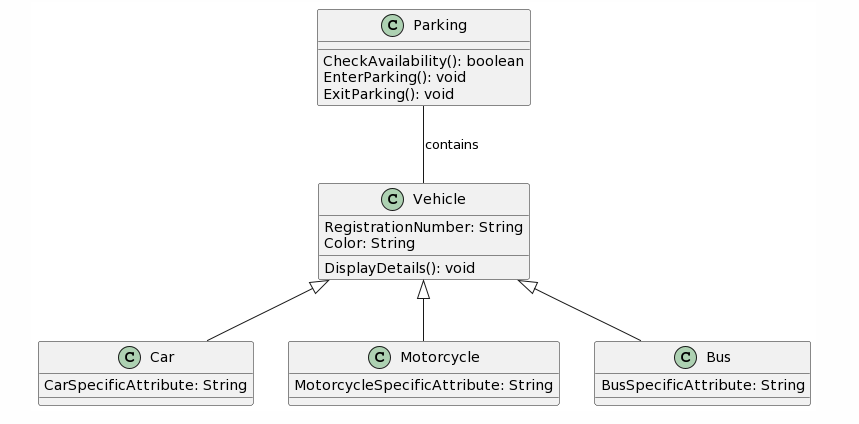
\includegraphics[width=0.75\textwidth]{photos/diagram.png}
\caption{Diagram klas systemu zarządzania parkingiem.}
\end{figure}

Struktura projektu jest zaprojektowana w taki sposób, aby maksymalizować ponowne wykorzystanie kodu i ułatwić rozszerzanie systemu o nowe funkcjonalności.
\section{Opis Techniczny Projektu}

\subsection{Wykorzystywany Język i Narzędzia}
Projekt został zrealizowany w języku C\#, co zapewnia szerokie możliwości w zakresie programowania obiektowego i zarządzania danymi. Do zarządzania projektem i kodem źródłowym wykorzystano środowisko Visual Studio Code z dodatkowymi wtyczkami, takimi jak PlantUML dla generowania diagramów klas UML, oraz Git jako system kontroli wersji.

\subsection{Minimalne Wymagania Sprzętowe}
System jest zaprojektowany z myślą o niskich wymaganiach sprzętowych, co czyni go dostępnym na większości współczesnych komputerów i serwerów. Minimalne wymagania to:
\begin{itemize}
    \item Procesor: 1 GHz lub szybszy.
    \item Pamięć RAM: 512 MB dla klienta, 2 GB dla serwera.
    \item Przestrzeń na dysku: 100 MB.
    \item System operacyjny: Windows 7 lub nowszy, Linux, MacOS.
\end{itemize}

\subsection{Zarządzanie Danymi i Baza Danych}
Projekt wykorzystuje mechanizm zarządzania danymi oparty na bazie danych w pliku tekstowym (txt), co pozwala na prostą i efektywną manipulację danymi bez potrzeby korzystania z zewnętrznych systemów DBMS. Taki wybór umożliwia łatwą portowalność i minimalizuje wymagania sprzętowe oraz konfiguracyjne. Struktura plików tekstowych jest zaprojektowana w taki sposób, aby umożliwić szybkie odczytywanie i zapisywanie stanu miejsc parkingowych oraz informacji o pojazdach, co zapewnia wysoką wydajność działania systemu.
\section{Harmonogram Realizacji Projektu}

Harmonogram realizacji projektu został zaplanowany z wykorzystaniem diagramu Gantta, który ilustruje kluczowe etapy rozwoju projektu, ich zależności czasowe oraz alokację zasobów. Poniżej przedstawiono diagram Gantta dla projektu System Zarządzania Parkingiem.

\begin{figure}[H]
\centering
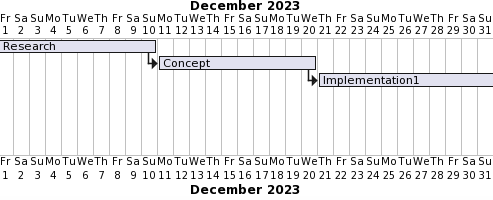
\includegraphics[width=\textwidth]{photos/gant1.png}
\caption{Diagram Gantta projektu System Zarządzania Parkingiem.}
\end{figure}
\begin{figure}[H]
\centering
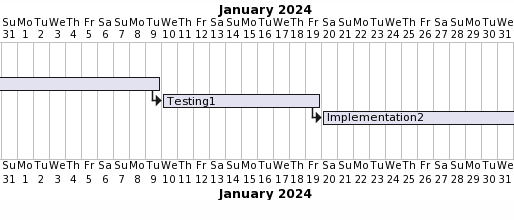
\includegraphics[width=\textwidth]{photos/gant2.png}
\caption{Diagram Gantta projektu System Zarządzania Parkingiem.}
\end{figure}
\begin{figure}[H]
\centering
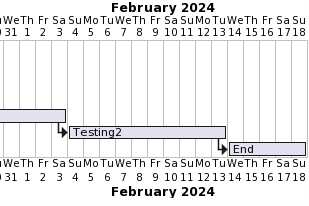
\includegraphics[width=\textwidth]{photos/gant3.png}
\caption{Diagram Gantta projektu System Zarządzania Parkingiem.}
\end{figure}
\section{Repozytorium i System Kontroli Wersji}

Projekt wykorzystuje system kontroli wersji Git, co umożliwia skuteczne zarządzanie historią zmian kodu źródłowego. Repozytorium kodu znajduje się na platformie GitHub pod adresem:\\ \url{https://github.com/filwalu/ProjektOOP} i będzie dostępne publicznie do dnia 30.09.2024. Bezpieczne\\ połączenie z repozytorium zabezpieczono za pomocą pary kluczy SSH. Poniżej przedstawiono opis\\ użytych poleceń Git:

\begin{enumerate}
    \item \texttt{git init} - inicjalizacja nowego repozytorium Git.
    \item \texttt{git clone [URL]} - klonowanie repozytorium przy użyciu SSH.
    \item \texttt{git add -Av} - dodawanie zmian do kolejki commitów.
    \item \texttt{git status} - sprawdzanie statusu zmian.
    \item \texttt{git commit -m "[wiadomość]"} - commitowanie zmian z opisem.
    \item \texttt{git push} - wysyłanie zmian do zdalnego repozytorium przez SSH.
\end{enumerate}

Zarządzanie projektem za pomocą Git pozwala na efektywne śledzenie postępów i zapewnia wysoki poziom bezpieczeństwa dzięki wykorzystaniu autoryzacji SSH.

\section{Prezentacja Warstwy Użytkowej Projektu}

Projekt Systemu Zarządzania Parkingiem oferuje intuicyjny i prosty w obsłudze interfejs użytkownika, który umożliwia szybkie zarządzanie miejscami parkingowymi oraz monitorowanie dostępności przestrzeni parkingowej. Interfejs użytkownika został zaprojektowany z myślą o zapewnieniu maksymalnej użyteczności i dostępności funkcji.

\subsection{Opis Aplikacji}
Aplikacja umożliwia użytkownikom wykonanie następujących akcji:
\begin{itemize}
    \item Sprawdzenie dostępności miejsc parkingowych.
    \item Rejestracja wjazdu i wyjazdu pojazdów.
    \item Zarządzanie danymi pojazdów.
    
\end{itemize}

Interfejs skupia się na minimalizmie i łatwości nawigacji, co pozwala na szybkie odnalezienie potrzebnych informacji i funkcji.

\subsection{Zrzuty Ekranu Aplikacji}
W tej sekcji zostaną umieszczone zrzuty ekranu przedstawiające kluczowe funkcjonalności aplikacji oraz jej interfejs użytkownika.

\begin{figure}[H]
\centering
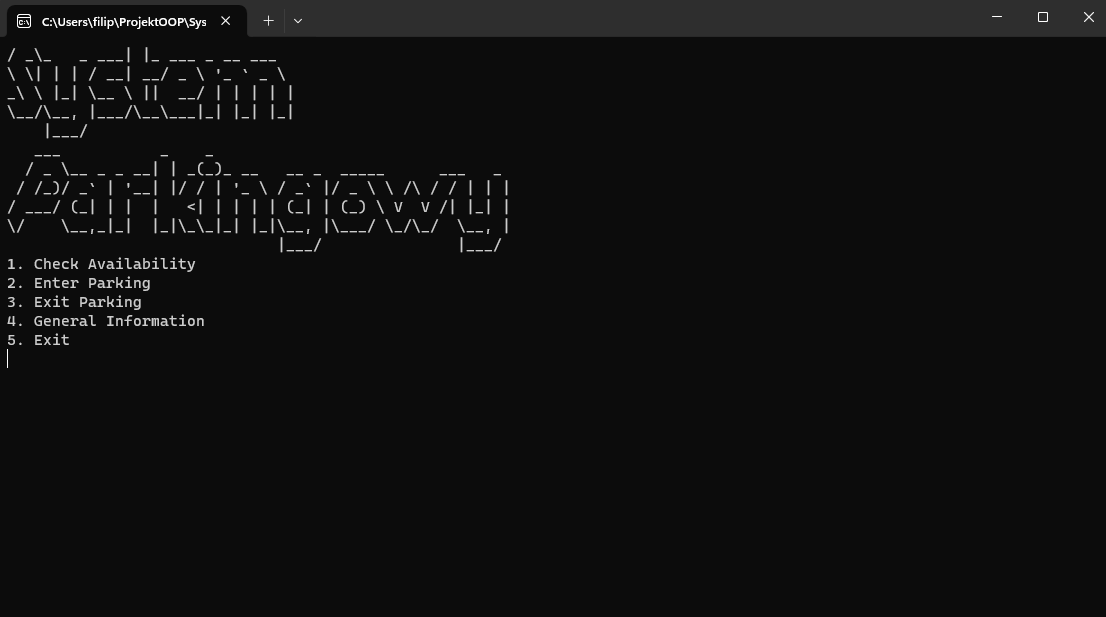
\includegraphics[width=\textwidth]{photos/mainmenu.png}
\caption{Widok głównego menu aplikacji.}
\end{figure}

\clearpage
\subsection{Nawigacja i Funkcjonalności}
W tej sekcji omówione zostaną kluczowe funkcjonalności aplikacji Systemu Zarządzania Parkingiem oraz instrukcje dotyczące ich używania.

\begin{itemize}
    \item \textbf{Sprawdzanie dostępności miejsc parkingowych} (\textit{Check Availability}):
    Użytkownik może sprawdzić dostępność miejsc parkingowych dla samochodów, wybierając opcję "1". 

    \begin{figure}[H]
    \centering
    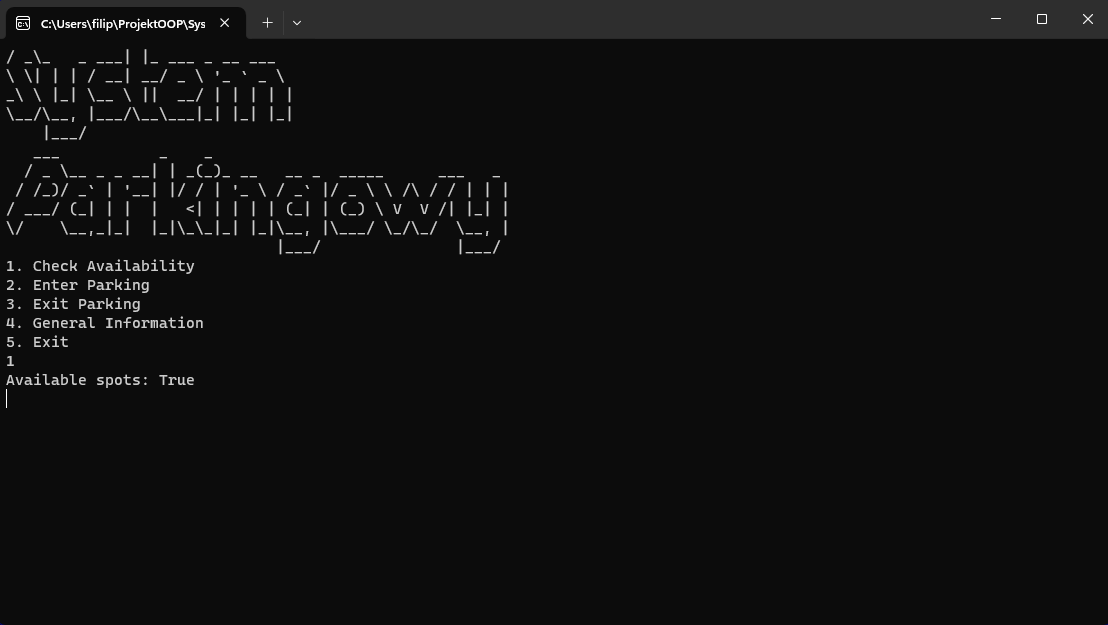
\includegraphics[width=\textwidth]{photos/avail.png}
    \caption{Opcja 1 - Check Availability.}
    \end{figure}

    \item \textbf{Wprowadzanie pojazdów na parking}:
    Użytkownik może wprowadzić pojazd na parking, wybierając opcję "2". Następnie należy podać numer rejestracyjny pojazdu, jego kolor oraz wybrać typ pojazdu (1 - Samochód, 2 - Motocykl, 3 - Autobus). Na podstawie podanych informacji, system tworzy odpowiedni obiekt pojazdu i rejestruje go w systemie parkingowym. 
        \begin{figure}[H]
        \centering
        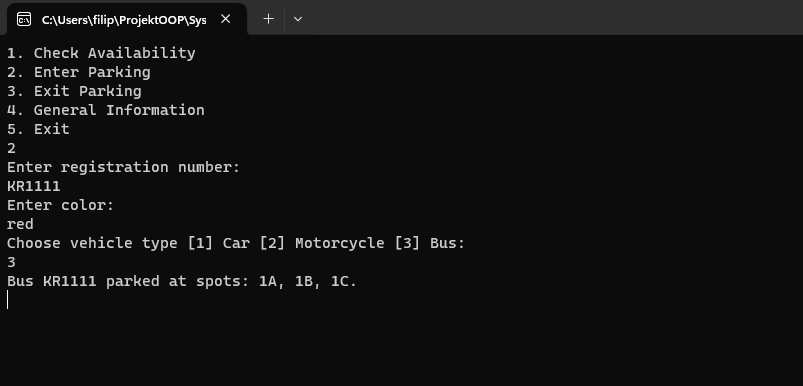
\includegraphics[width=\textwidth]{photos/enter.png}
        \caption{Opcja 2 - Enter Parking.}
        \end{figure}
    \clearpage
    \item \textbf{Wyjazd pojazdów z parkingu}:
    Użytkownik może wyjechać pojazdem z parkingu, wybierając opcję "3". Następnie należy podać numer rejestracyjny pojazdu. Na podstawie podanej informacji, system usuwa pojazd z rejestru parkingowego. 
    \begin{figure}[H]
        \centering
        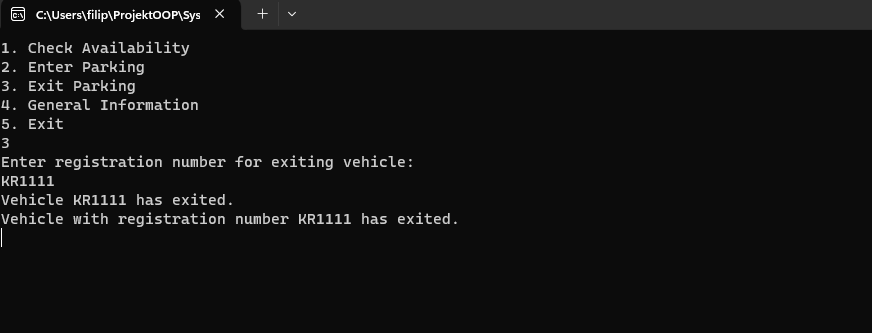
\includegraphics[width=\textwidth]{photos/exit.png}
        \caption{Opcja 3 - Exit Parking.}
        \end{figure}
    \item \textbf{Dodatkowe informacje}:
    Użytkownik wybierając opcję "4"\ wyświetla dodatkowe informacje o systemie.
        \begin{figure}[H]
        \centering
        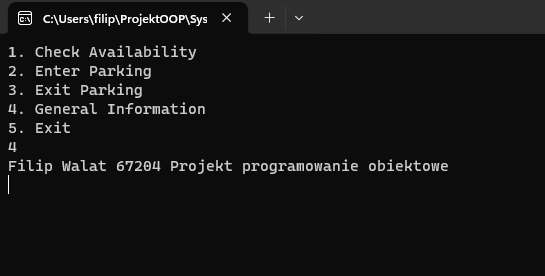
\includegraphics[width=\textwidth]{photos/info.png}
        \caption{Opcja 4 - General Information.}
        \end{figure} 
\item \textbf{Koniec}:
    Użytkownik wybierając opcję "5"\ zamyka aplikacje.
\clearpage
\subsection{Interakcja z Użytkownikiem}
Sekcja ta zawiera informacje na temat interakcji z użytkownikiem, w tym otrzymywanych komunikatów, alertów oraz sposobu obsługi błędów. Poniżej przedstawiono wybrane komunikaty wyświetlane przez aplikację:

\begin{itemize}
    \item \texttt{"Available spots: [True lub False]"} - informacja mówiąca czy znajdują się obecnie wolne miejsca parkingowe.
    \item \texttt{"Enter registration number:"} - monit o wprowadzenie numeru rejestracyjnego pojazdu.
    \item \texttt{"Enter color:"} - prośba o podanie koloru pojazdu.
    \item \texttt{"Choose vehicle type [1] Car [2] Motorcycle [3] Bus:"} - wybór typu pojazdu do wprowadzenia na parking.
    \item \texttt{"Invalid vehicle type selected."} - komunikat o błędnym wyborze typu pojazdu.
    \item \texttt{"Vehicle entered the parking."} - informacja o pomyślnym wprowadzeniu pojazdu na parking.
    
    
\end{itemize}


\section{Podsumowanie}

\subsection{Zrealizowane Prace}
W ramach projektu Systemu Zarządzania Parkingiem wykonano szereg prac, w tym:
\begin{itemize}
    \item Projektowanie i implementacja klas reprezentujących pojazdy (samochody, motocykle, autobusy) oraz parking.
    \item Rozwój funkcjonalności zarządzania miejscami parkingowymi, w tym sprawdzanie dostępności, rejestracja wjazdu i wyjazdu pojazdów.
    
    \item Przygotowanie interfejsu użytkownika w konsoli do interakcji z systemem.
    \item Wykorzystanie plików tekstowych do prostego zarządzania danymi.
\end{itemize}

\subsection{Planowane Prace Rozwojowe}
W dalszej kolejności planowane są następujące prace rozwojowe:
\begin{itemize}
    \item Zastosowanie klasycznej bazy danych SQL, np. PostgreSQL, dla lepszego zarządzania danymi i wydajności.
    \item Konteneryzacja aplikacji z wykorzystaniem Docker, co ułatwi wdrożenie i skalowalność.
    \item Implementacja systemu płatności 
    \item Usprawnienia interfejsu użytkownika, w tym rozwój graficznego interfejsu użytkownika (GUI) dla lepszej dostępności i ergonomii.
    \item Rozbudowa obsługi wyjątków dla zwiększenia stabilności i niezawodności aplikacji.
    \item Implementacja możliwości generowania raportów w formacie CSV z danych przechowywanych w systemie dla ułatwienia analizy i zarządzania.
\end{itemize}
\clearpage 
\listoffigures 

\clearpage 
\begin{thebibliography}{9}

\bibitem{gitpro}
Scott Chacon, Ben Straub. \textit{Pro Git}. Apress, 2014. Dostępne online: \url{https://git-scm.com/book/en/v2}

\bibitem{dotnetdocs}
Dokumentacja Microsoft .NET. Microsoft, dostęp online: \url{https://docs.microsoft.com/en-us/dotnet/}



\bibitem{csharpstudy}
Albahari, Joseph, Albahari, Ben. \textit{C\# 7.0 in a Nutshell: The Definitive Reference}. O'Reilly Media, 2017.

\end{thebibliography}


\end{document}
